% Drawing 76/01-1 -- folder 76, batch 01, archive page 11 (PDF page 12).
% Transcription: figure : le treillis des drapeaux pour $n = 2$. En haut $D_{012}$ ; de lui descendent des flèches vers $D_{01}$, $D_{02}$, $D_{12}$, marquées « épi » ; de ceux-ci vers $D_0$, $D_1$, $D_2$, la flèche $D_{02} \to D_1$ barrée d'une croix, et « épi » sur plusieurs flèches
% Kind: lattice of flags for n = 2. Method 2 (schematic redraw from the facsimile). Status: partial.
% Notes: D012 on top, arrows down to D01, D02, D12 ("épi" beside), and from these to D0, D1, D2; two crossing strokes (crosses) on lower arrows are drawn where they stand: the transcription puts the cross on D02 -> D1, on the crop one cross stands between D02 and D1 and another between D12 and D2, which arrow each strikes is a reading. Above the lattice, "D01 épi !!" with arrows to D0 and D1 and a long underline are not drawn (text of the page).
% Coordinates: 1 unit = 1 mm = 1/100 of the crop width (bbox in page fractions: [0.42, 0.2, 0.7, 0.36]).
% Redrawn by Claude (claude-opus-5-5), issue #73, 2026-11-07; not checked by a human; not compiled (no TeX in the session).
% Rights: reproduces part of the work -- behind RENDER_TRANSCRIPTS, never published by itself.
\documentclass[tikz,border=3pt]{standalone}
\usepackage{amsmath,amssymb}
\usetikzlibrary{patterns,arrows.meta}
\tikzset{pencil/.style={black!45}, struck/.style={black!35}, mark/.style={circle,draw,inner sep=1.3pt}, pt/.style={circle,fill,inner sep=0.9pt}, opt/.style={circle,draw,fill=white,inner sep=1.1pt}}
\begin{document}
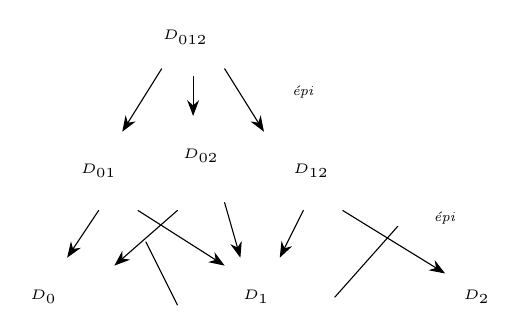
\begin{tikzpicture}[x=1mm,y=1mm,line cap=round,line join=round,font=\scriptsize]
\node[inner sep=1pt] at (51,-40) {\tiny $D_{012}$};
\node[inner sep=1pt] at (40,-57) {\tiny $D_{01}$};
\node[inner sep=1pt] at (53,-55) {\tiny $D_{02}$};
\node[inner sep=1pt] at (67,-57) {\tiny $D_{12}$};
\node[inner sep=1pt] at (33,-73) {\tiny $D_0$};
\node[inner sep=1pt] at (60,-73) {\tiny $D_1$};
\node[inner sep=1pt] at (88,-73) {\tiny $D_2$};
\node[inner sep=1pt] at (66,-47) {\tiny \textit{épi}};
\node[inner sep=1pt] at (84,-63) {\tiny \textit{épi}};
\draw[-{Stealth[length=2mm]}] (48,-44) -- (43,-52);
\draw[-{Stealth[length=2mm]}] (52,-45) -- (52,-50);
\draw[-{Stealth[length=2mm]}] (56,-44) -- (61,-52);
\draw[-{Stealth[length=2mm]}] (40,-62) -- (36,-68);
\draw[-{Stealth[length=2mm]}] (45,-62) -- (56,-69);
\draw[-{Stealth[length=2mm]}] (50,-62) -- (42,-69);
\draw[-{Stealth[length=2mm]}] (56,-61) -- (58,-68);
\draw[-{Stealth[length=2mm]}] (66,-62) -- (63,-68);
\draw[-{Stealth[length=2mm]}] (71,-62) -- (84,-70);
\draw (46,-66) -- (50,-74);
\draw (70,-73) -- (78,-64);
\end{tikzpicture}
\end{document}
